\chapter{User Guide}
Before deploying and running the system, certain prerequisites must be met to ensure a successful setup process. One of the primary requirements is the installation of Docker, which serves as the foundation for creating and managing the application's containers.
\newline
\\
For reference and reproducibility, the complete implementation described in this thesis is available in the accompanying source code repository: 
\url{https://github.com/rileydavid/kraken-lstm-prediction-engine}

\section{Prerequisites}

\subsection{Docker Installation}
To run this application, Docker must be installed and properly configured. The following steps have to be successfully completed:

\begin{enumerate}
    \item \textbf{Download Docker}: Visit the official Docker website at \url{https://www.docker.com/get-started} and download the appropriate Docker Desktop application for your operating system.
    \item \textbf{Install Docker}: Execute the installer and follow the on-screen instructions to install Docker on your machine. Ensure that the neeeded administrative privileges are available to complete the installation.
    \item \textbf{Verify Installation}: Open a terminal or command prompt and run the command \texttt{docker ---version} to verify that Docker has been installed correctly. The Docker version number should show up in the output.
    \item \textbf{Post-Installation Steps}: Depending on the host operating system, there may be additional post-installation steps required. These are detailed in the Docker documentation and ensure that Docker runs smoothly.
\end{enumerate}

\subsection{Historical Dataset}
\label{section:historical_dataset}
To make sure the frontend is fully functional and to enable predictions the historical data for the currency pair \texttt{ETH/USD} is needed, which can be downloaded from \url{https://support.kraken.com/hc/en-us/articles/360047543791-Downloadable-historical-market-data-time-and-sales-}. Download the full dataset as well as the incremental update for 2023 Q3 and optionally Q4. 

\section{Starting the Application}

To start the application, follow the steps below. Ensure you are in the root directory of the project, where the \texttt{docker-compose.yaml} file is located.

\begin{enumerate}
\item \textbf{Start Docker:} Run the following command in a terminal or command prompt:
\begin{verbatim}
docker-compose --env-file config.env up --build
\end{verbatim}
This will build all necessary container images and start them afterwards. This process might take a while as it is pulling in dependencies and compiling the source code. 

\item \textbf{Access MinIO Dashboard:} Navigate to the MinIO dashboard at \url{http://172.1.0.12:2001/}. Log in using the credentials from the \texttt{config.env} file. The default credentials are:
\begin{verbatim}
MINIO_ROOT_USER=minio_root_user
MINIO_ROOT_PASSWORD=minio_password
\end{verbatim}

\item \textbf{Create a Bucket:} Create a bucket named \texttt{prod-model} (Figure \ref{fig:minio_create_bucket}).

\begin{figure}[ht!]
    \centering
    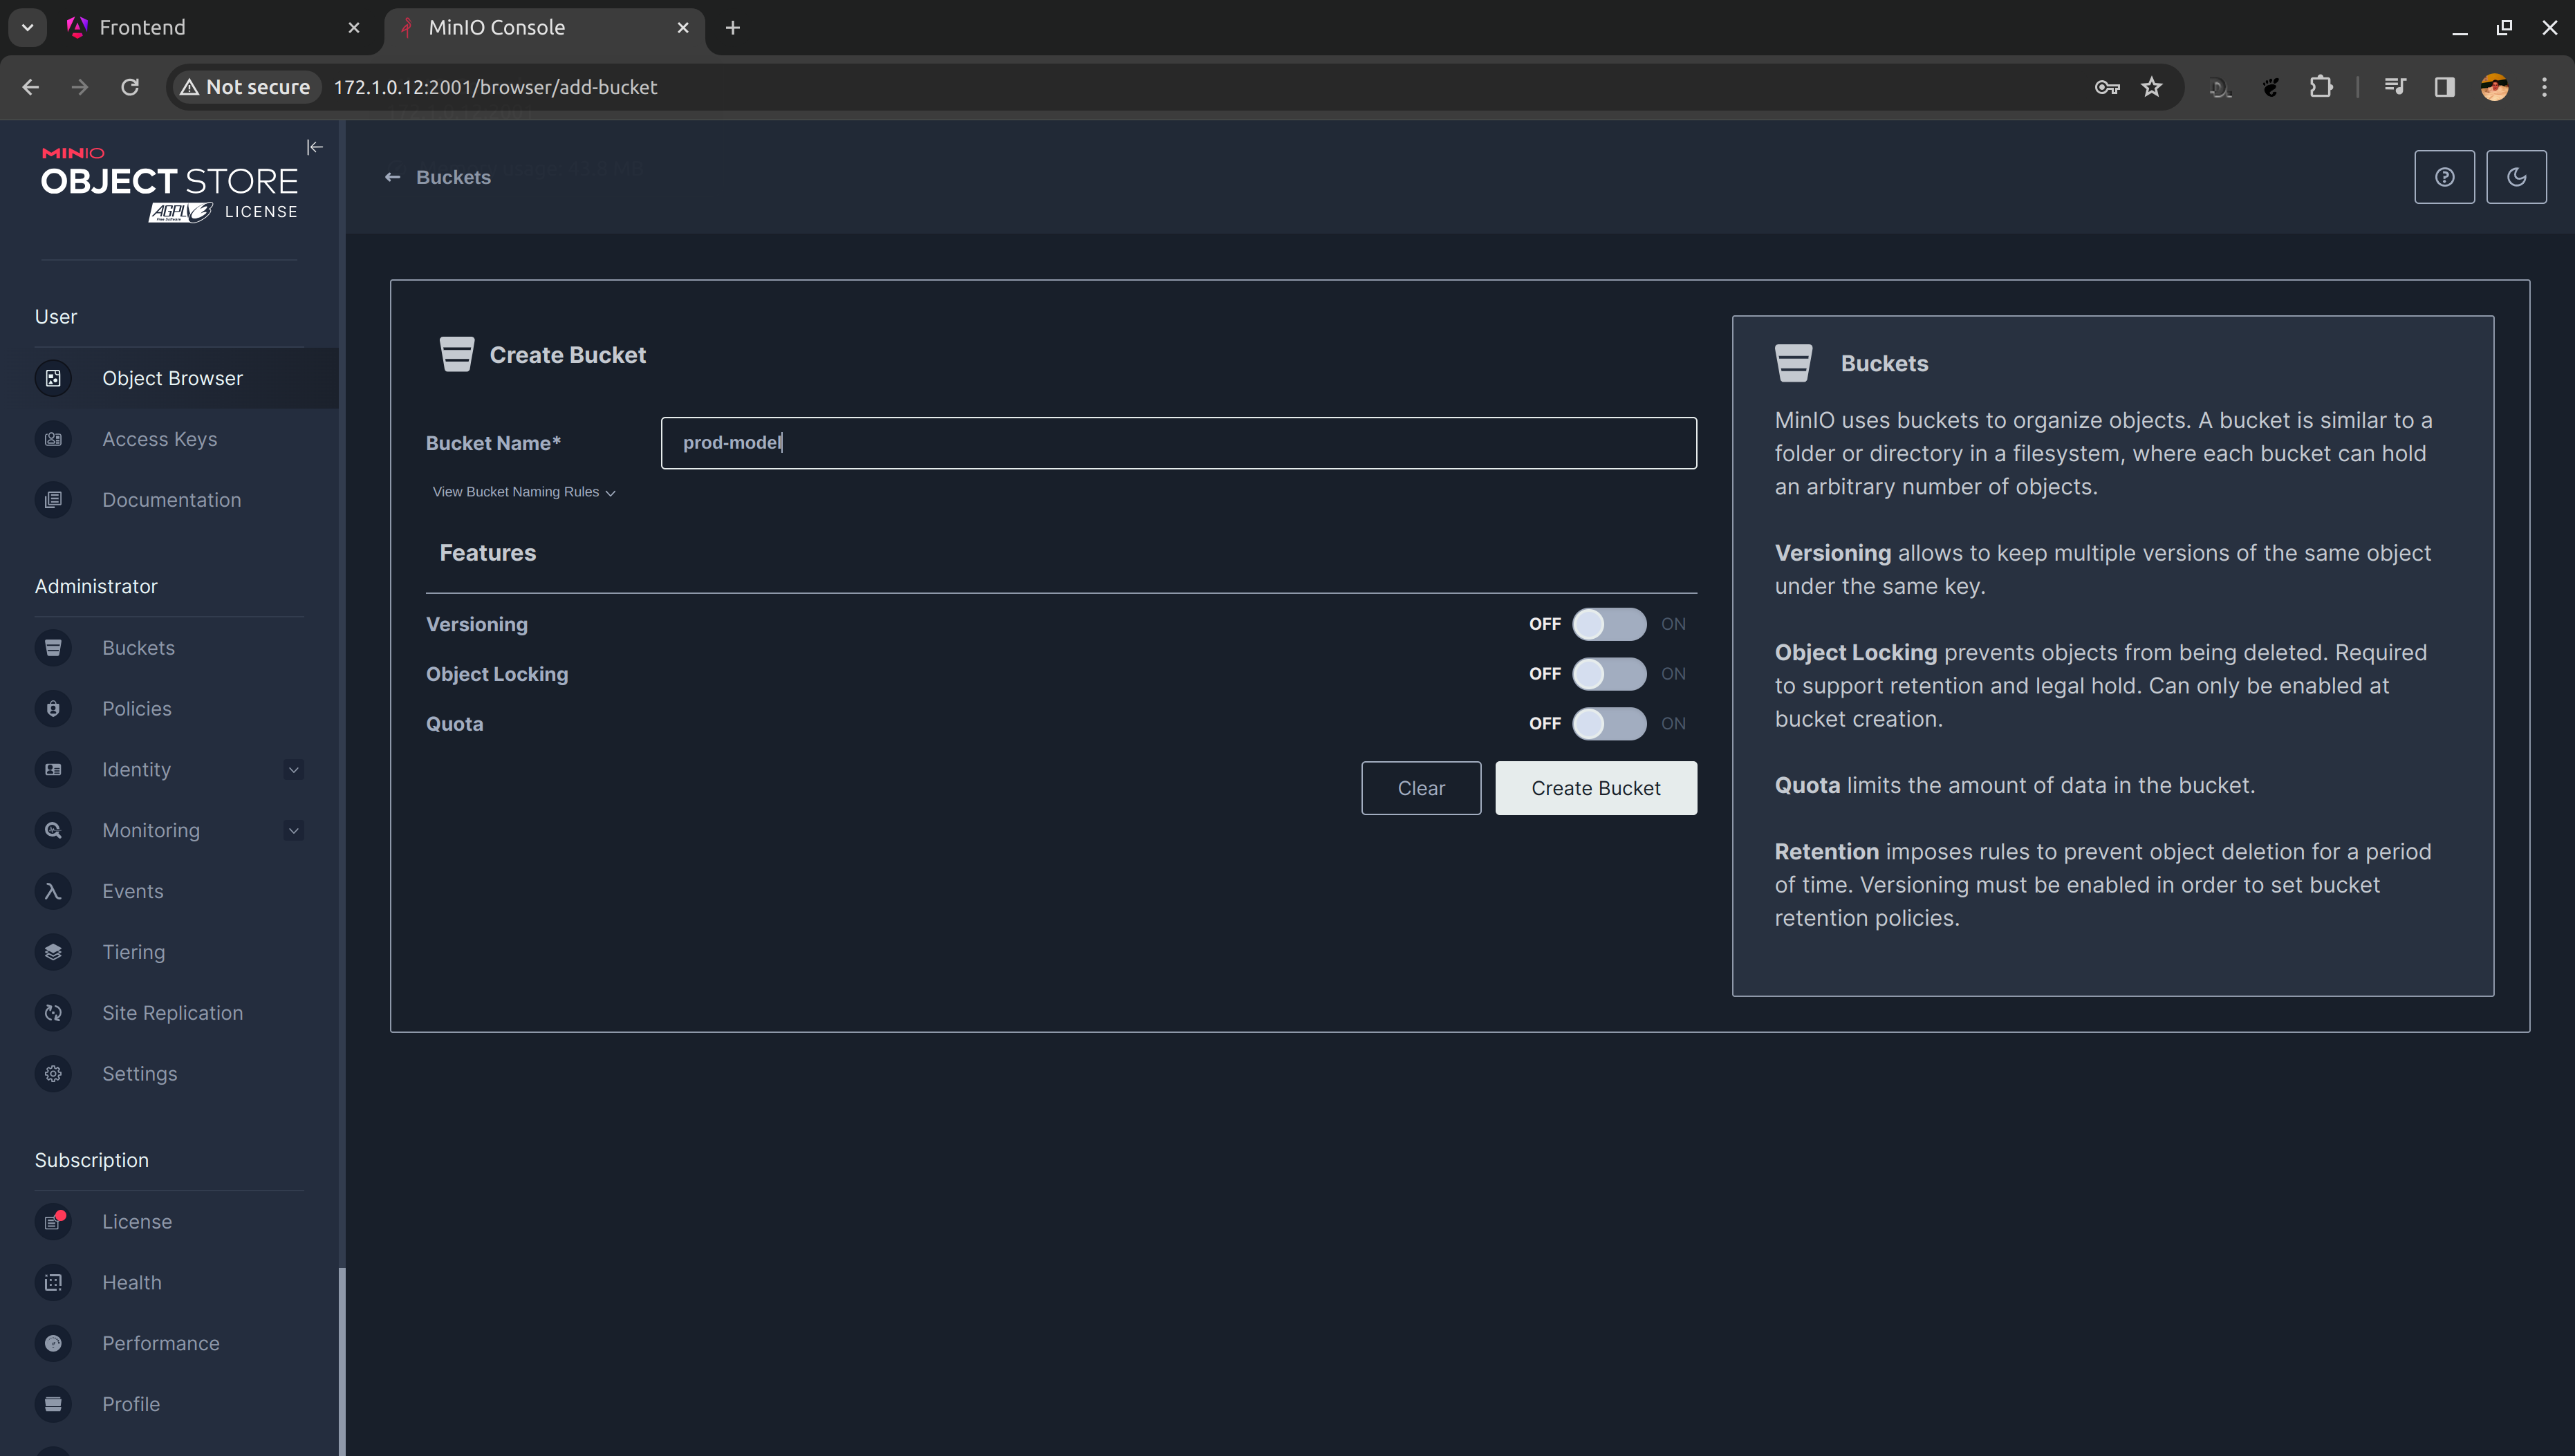
\includegraphics[width=\textwidth]{figures/create_bucket.png}
    \caption{Create Bucket in Minio}
    \label{fig:minio_create_bucket}
\end{figure}

\item \textbf{Upload Model File:} Upload the \texttt{clean-mare-368.pkl} file from the \texttt{data/model} folder to the \texttt{prod-model} bucket.

\item \textbf{Update Access Keys:} Create new access keys (Figure \ref{fig:minio_create_accesskeys}) and update them in the \texttt{config.env} file:
\begin{verbatim}
MINIO_ACCESS_KEY=eITEO5kyE7hccuy7UTHv
MINIO_SECRET_ACCESS_KEY=5KBCscit30Z70bSVGIMvMBBoqV8ydn232o2MW9RA
\end{verbatim}

    \begin{figure}[H]
    \centering
    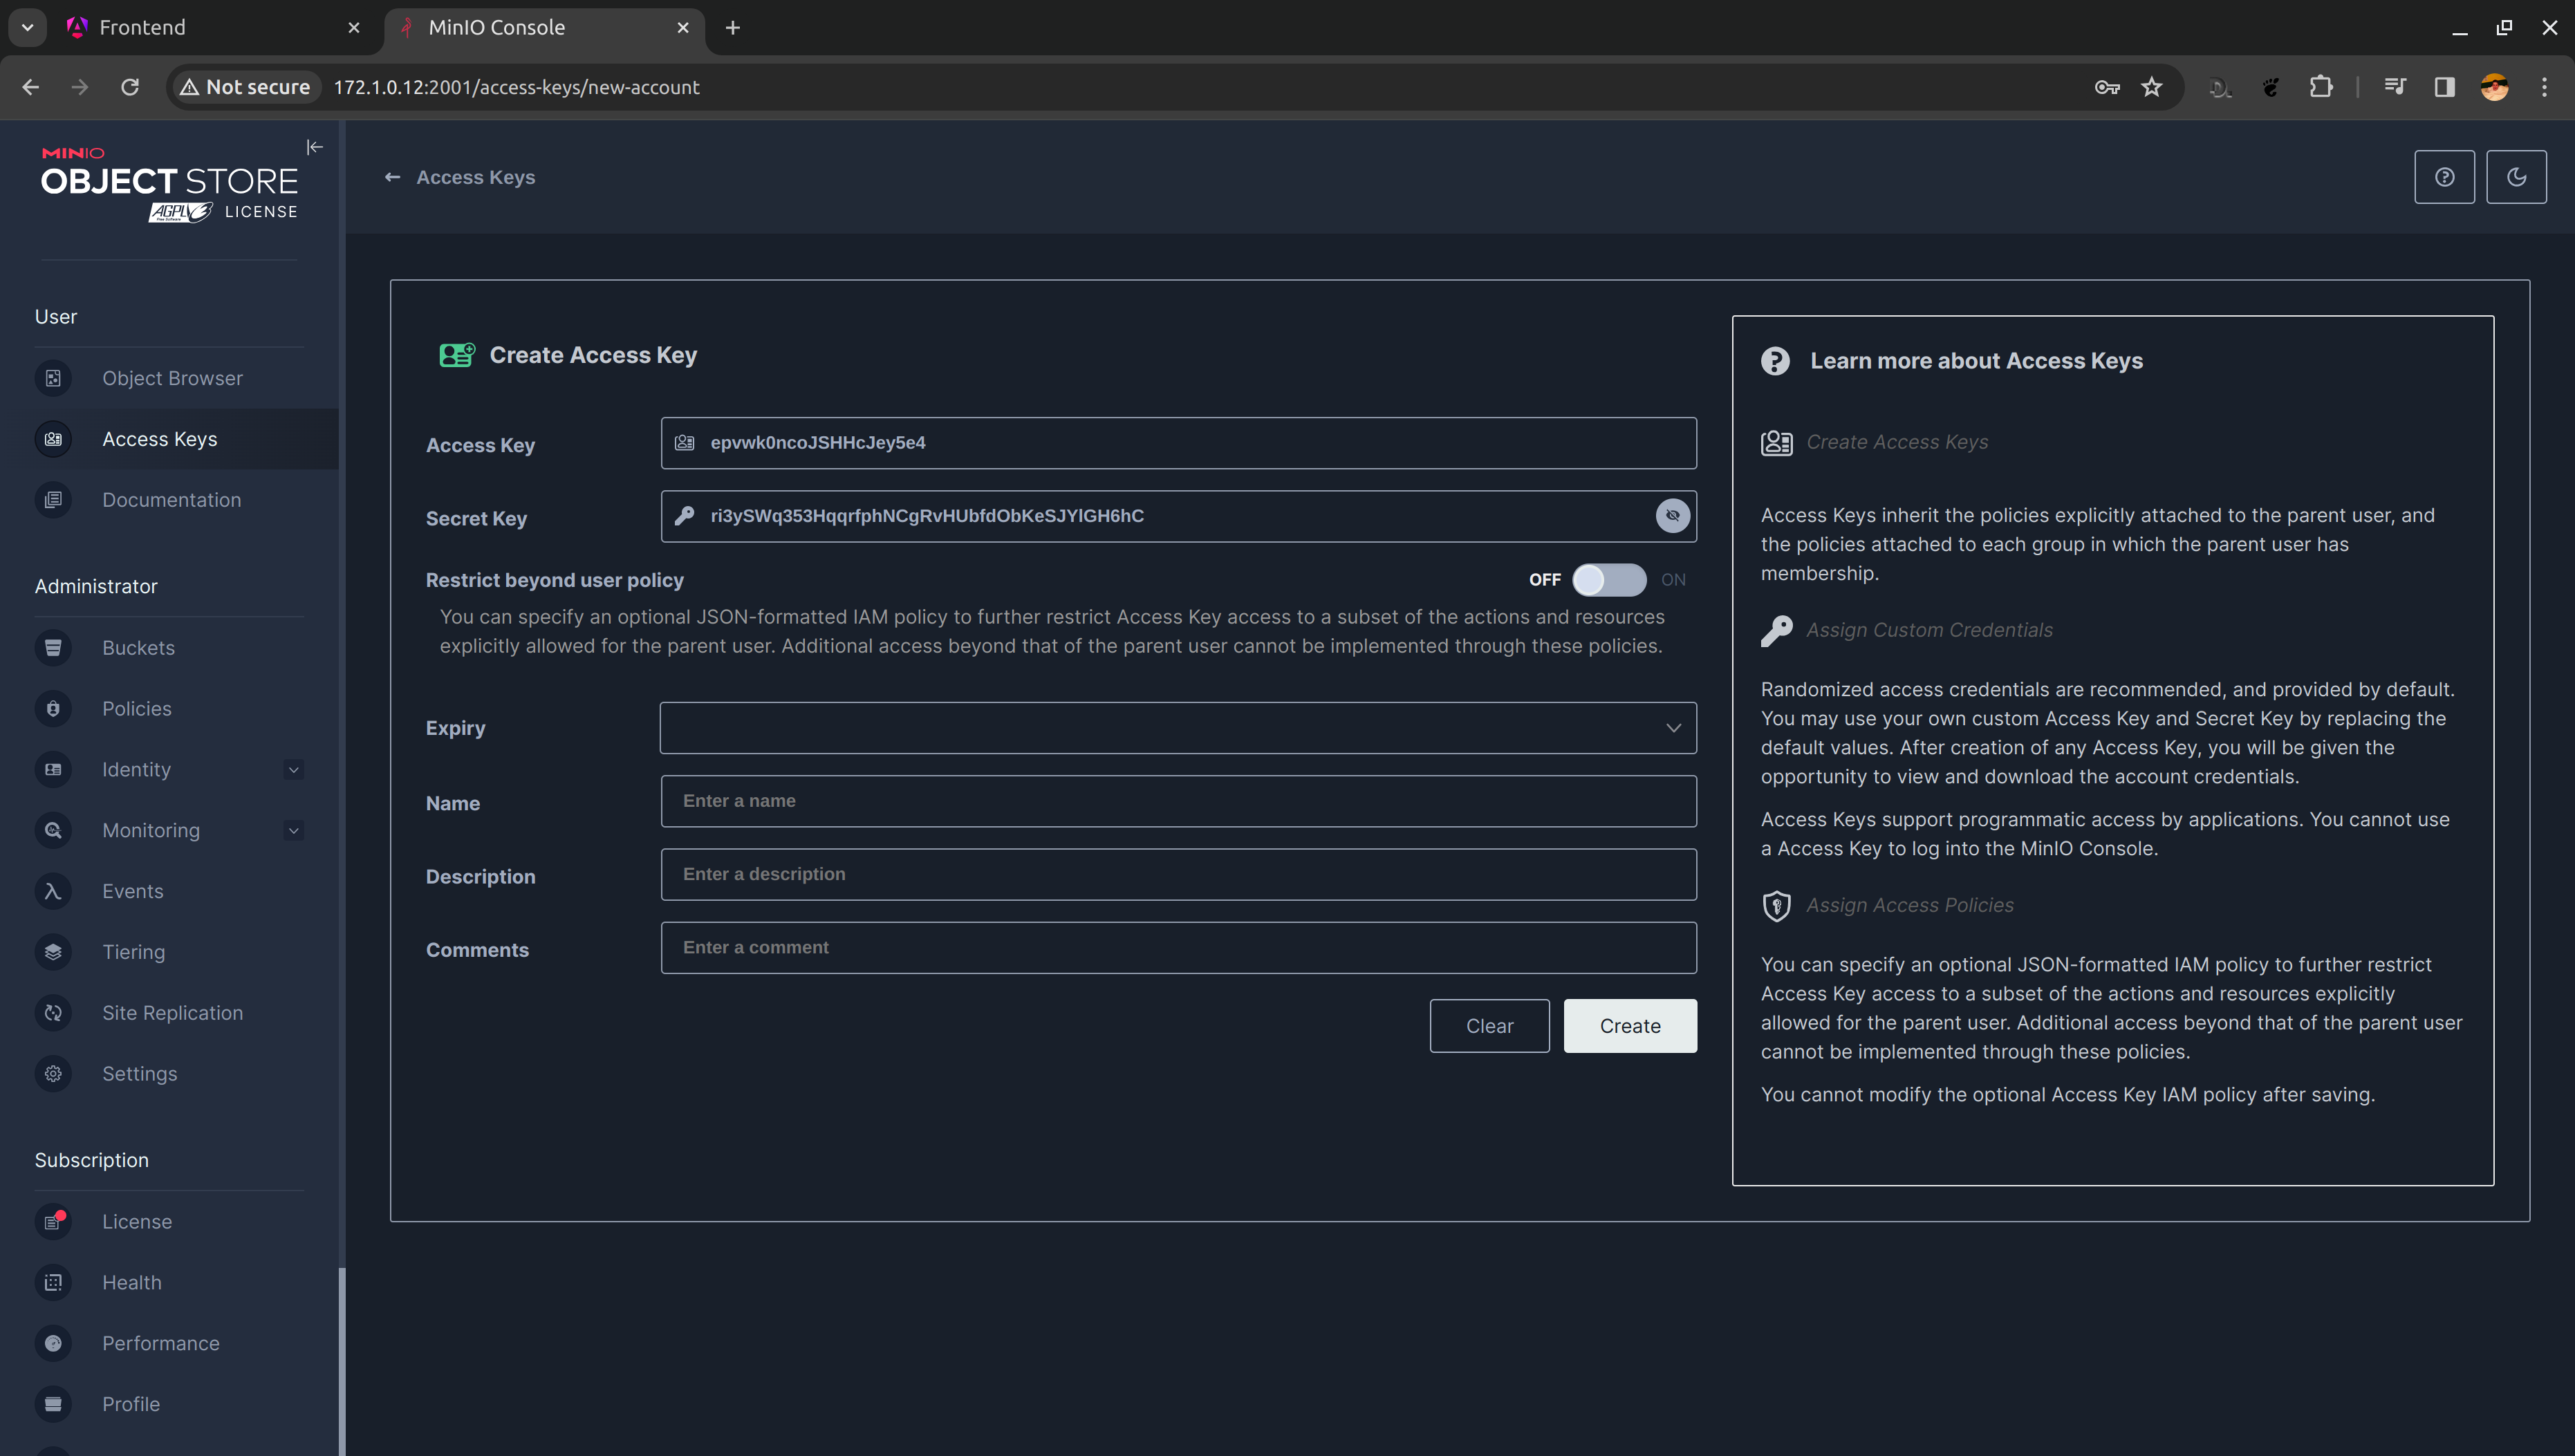
\includegraphics[width=\textwidth]{figures/accesskey_generate.png}
    \caption{Create Access Keys in Minio}
    \label{fig:minio_create_accesskeys}
\end{figure}

\item \textbf{Restart Docker:} Execute the following commands to restart the services:
\begin{verbatim}
docker-compose --env-file config.env down
docker-compose --env-file config.env up --build
\end{verbatim}

\item \textbf{Open Frontend:} After the docker containers have started, open the frontend in a browser: \url{http://localhost:4200}.

\item \textbf{Upload:} Navigate to the \texttt{Upload} tab on the Frontend and upload the historical data for \text{ETH/USD} (Section \ref{section:historical_dataset})

\item \textbf{Import:} To import the just uploaded .csv files navigate to the \texttt{Import} tab and import the necessary files by entering the sybmol \texttt{ETH} and start the import using the import button. Currently it is only possible to add USD currency pairs as the backend automatically fills in the USD part.  

\item \textbf{Dashboard: } Now the main functionality of the system is ready. Try it out by navigating to the Dashboard and selecting the \texttt{ETH/USD} symbol and press fetch.
\end{enumerate}

\section{Model Tuning (Optional)}
To run the Model-tuning Script all libraries used have to be installed locally. \\

\begin{table}[H]
\centering
\begin{tabular}{ll}
\hline
\textbf{Name}         & \textbf{Version} \\ \hline
Python Kernel & 3.10.12      \\
numpy         & 1.23.5       \\
pandas        & 1.5.2        \\
more-itertools & 9.0.0       \\
mlflow        & 2.8.0        \\
keras         & 2.14.0       \\
ipython       & 8.7.0        \\
matplotlib    & 3.6.2        \\
scikit-learn  & 1.1.3        \\
holidays      & 0.32         \\ \hline
\end{tabular}
\caption{Software and Libraries Version List}
\label{tab:software_version}
\end{table}

Additionally it can be beneficial to install Nvidia CUDA \cite{NVIDIACUDAToolkit} to improve training performance, keep in mind that this is only a viable option if a Nvidia GPU is installed in the system. To run the model-tuning script (located in the \texttt{prediction-model-development} folder), replace the \texttt{AWS\_ACCESS\_KEY\_ID} and the \texttt{AWS\_SECRET\_ACCESS\_KEY} with the generated MinIO keys from earlier. The dataset required is available in the folder and therefore does not have to be exported using PgAdmin. \\
\begin{verbatim}
os.environ["AWS_ACCESS_KEY_ID"] = "eITEO5kyE7hccuy7UTHv"
os.environ["AWS_SECRET_ACCESS_KEY"] = "5KBCscit30Z70bSVGIMvMBBoqV8ydn232o2MW9RA"
\end{verbatim}

\section{PgAdmin}
\label{section:pgadmin_user_guide}
\subsection{Login and Configuration}
To make use of the export feature of \texttt{PgAdmin} navigate to \url{http://localhost:5050/} and login using the credentials configured in the \texttt{config.env} file (Section \ref{docker_config_env}). The landing page of \texttt{PgAdmin} (Figure \ref{fig:pgadmin_landing_page}) should open. 

\begin{figure}[H]
    \centering
    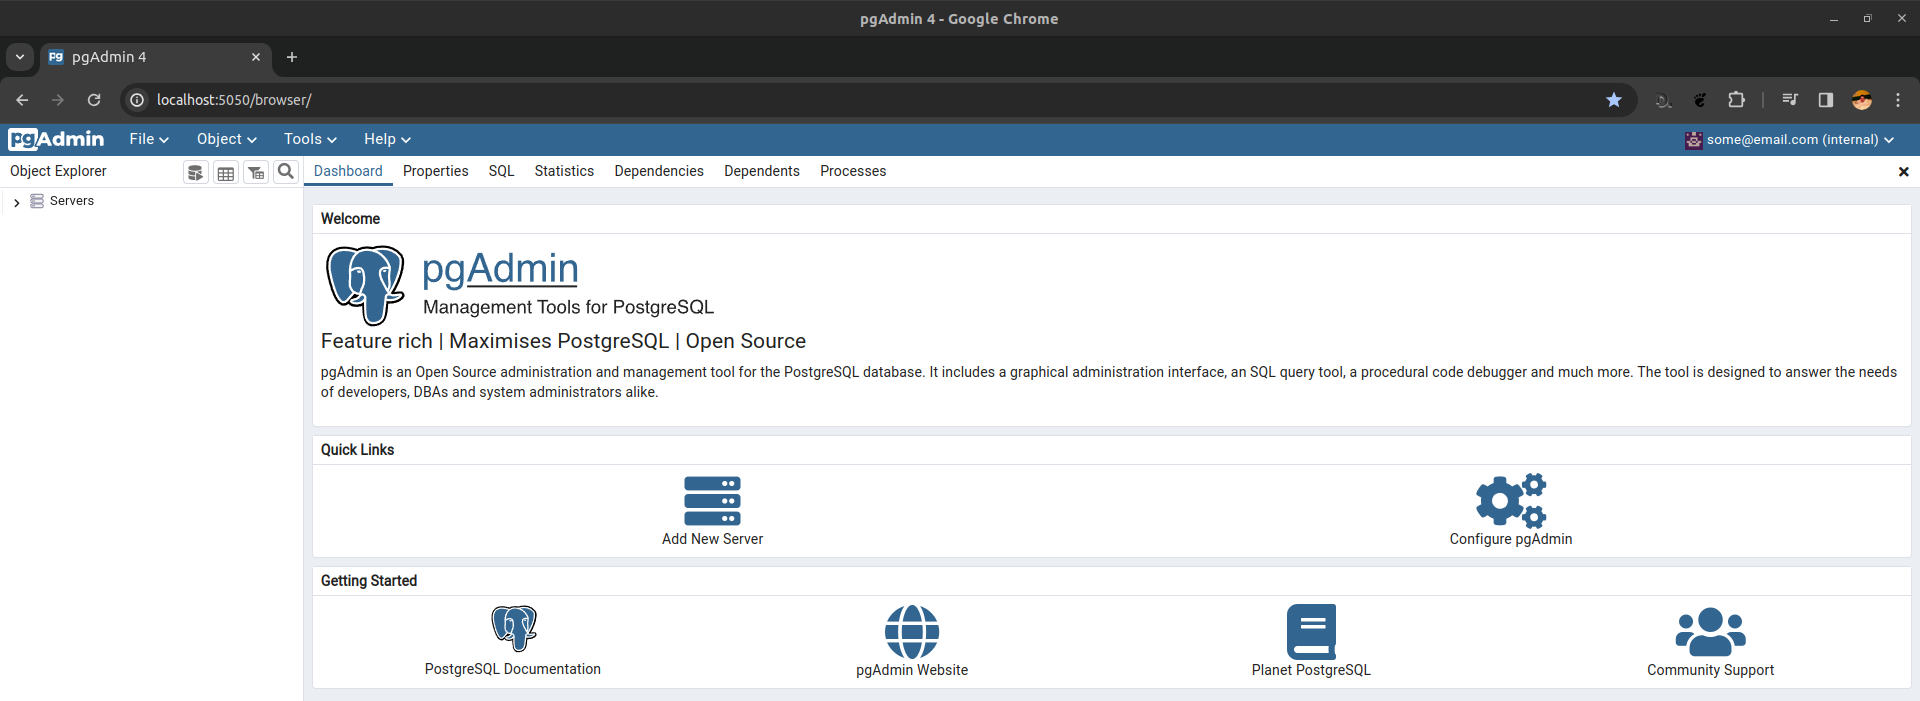
\includegraphics[width=\textwidth]{figures/pgadmin_landing_page.png}
    \caption{PgAdmin Dashboard}
    \label{fig:pgadmin_landing_page}
\end{figure}

On the landing page (Figure \ref{fig:pgadmin_landing_page}) press the add new server button. A dialog (Figure \ref{fig:pgadmin_add_server_page}) should open up. Enter a fitting name (e.g. \texttt{timescale}) and navigate to the \texttt{Connection} tab. 

\begin{figure}[H]
    \centering
    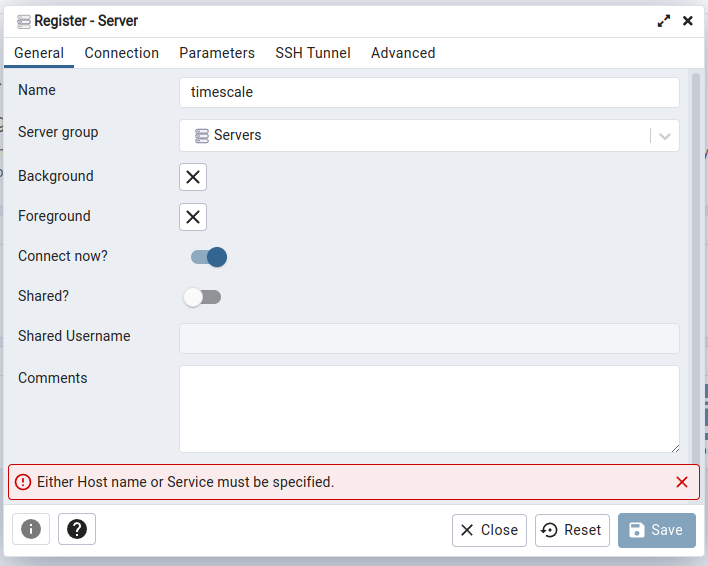
\includegraphics[width=0.75\textwidth]{figures/pgadmin_add_server_page.png}
    \caption{PgAdmin Add Server Dialog}
    \label{fig:pgadmin_add_server_page}
\end{figure}

After navigating to the \texttt{Connection} tab (Figure \ref{fig:pgadmin_server_ip_setup}) enter the IP-Address of timescale, \texttt{172.1.0.10}, if the default configuration has not been adapted. Enter the user and password for timescale, the default values are \texttt{admin} and \texttt{password} (Section \ref{docker_config_env}), and press save.  
\begin{figure}[H]
    \centering
    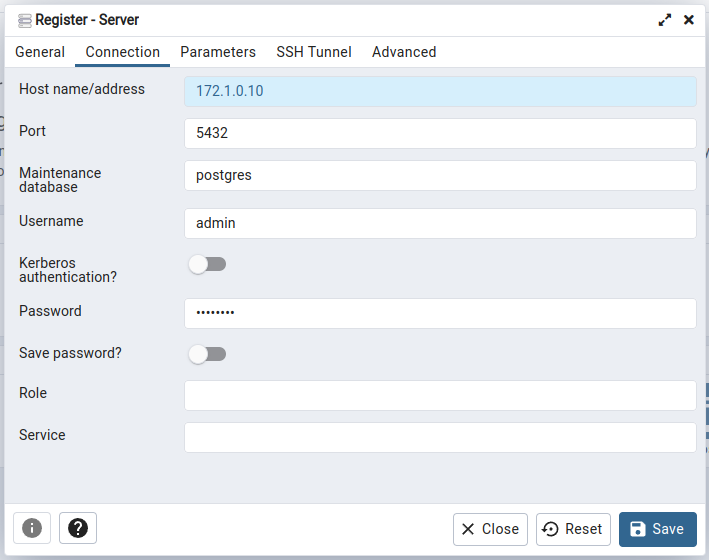
\includegraphics[width=\textwidth]{figures/pgadmin_server_ip_setup.png}
    \caption{PgAdmin Connection Tab}
    \label{fig:pgadmin_server_ip_setup}
\end{figure}

\subsection{Exporting Data}
To export data for training purposes press the \texttt{Tools} option in the menu bar and select the query tool (Figure \ref{fig:pgadmin_export}). Use the query text-field to run the following query (Listing \ref{lst:pg_query}): 

\begin{lstlisting}[language=sql, caption={ETH/USD Training Dataset Query}, label={lst:pg_query}]
SELECT * FROM ohlc_hour 
    WHERE symbol_id = 1 
    AND bucket >= '2020-01-01 00:00:00+00' 
    AND '2023-09-30 23:00:00+00' >= bucket 
    ORDER BY bucket ASC;
\end{lstlisting}

In the data output section use the download button to download this dataset as a .csv. 
\newpage
\begin{figure}[H]
    \centering
    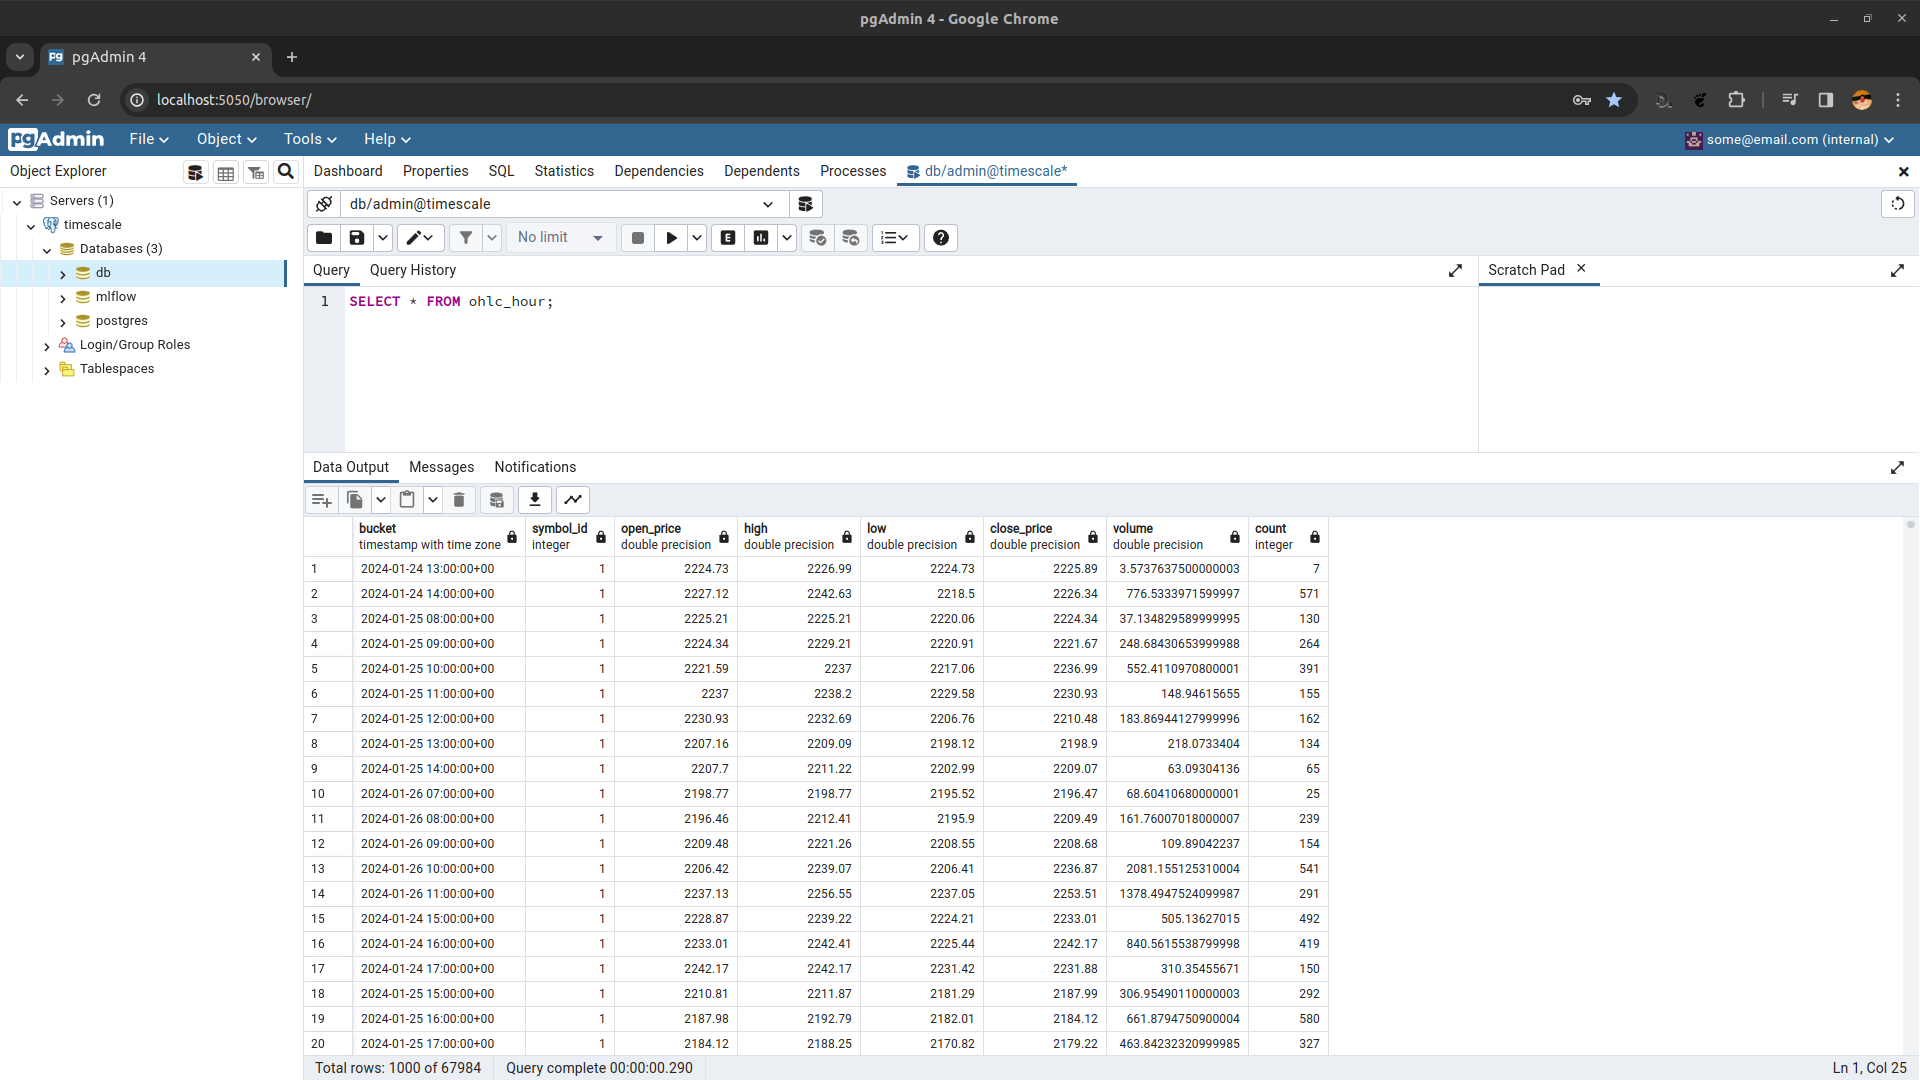
\includegraphics[width=\textwidth]{figures/pgadmin_export.png}
    \caption{PgAdmin Export}
    \label{fig:pgadmin_export}
\end{figure}

